\documentclass[a4paper, 12pt]{article}

% This file contains global setup commands so that we can write in our main document without cluttering up the workspace. This file is the first thing included in the main paper after the \documentclass command, and all settings are immediately available.

\usepackage{graphicx}
\usepackage{xcolor}
\usepackage{parskip}
\usepackage{wrapfig}
\usepackage{amsmath}

% Font settings
\usepackage{fontspec}
\usepackage{titlesec}
\usepackage{titling}
\setmainfont{Open Sans}
\newfontfamily \headingfont[]{Open Sans Light}
\newfontfamily \codefont[NFSSFamily=JetBrainsMono]{JetBrains Mono}
\definecolor{accent}{rgb}{0.8, 0.0, 0.0}
\titleformat{\section}
	{\Huge\headingfont}{\thesection}{1em}{}[{\color{accent}\titlerule[4pt]}]
\titleformat{\subsection}
	{\Large\headingfont}{\thesection}{1em}{}[{\color{accent}\titlerule[2pt]}]
\titleformat{\subsubsection}
	{\large\headingfont}{\thesection}{1em}{}[{\color{accent}\titlerule[1pt]}]
\setmonofont{JetBrains Mono}
% Set to clear page before each section.
\newcommand{\sectionbreak}{\clearpage}

% Link settings
\usepackage{hyperref}
\definecolor{linkcolour}{rgb}{0.7, 0.133, 0.133}
\hypersetup{
	colorlinks,
	breaklinks,
	urlcolor=linkcolour,
	linkcolor=linkcolour,
	citecolor=linkcolour
}

% Code settings
\usepackage{minted}
\usepackage[htt]{hyphenat}

% Note: For some reason, this patch is needed to allow minted to work with python3, since it just looks for "python" by default.
\usepackage{xpatch}
\makeatletter
\xpatchcmd\minted@pygmentize
	{python -c}
	{python3 -c}
	{}{\fail}
\xpatchcmd\minted@autogobble
	{python -c}
	{python3 -c}
	{}{\fail}
\makeatother

\usemintedstyle{default}
\definecolor{codebg}{rgb}{0.973, 0.973, 0.973}
\definecolor{codehighlight}{rgb}{0.360, 0.215, 0.309}
\setminted{
	autogobble=true,
	encoding=utf-8,
	numbers=left,
	bgcolor=codebg,
	highlightcolor=codehighlight,
	fontfamily=JetBrainsMono,
	fontsize=\scriptsize,
	breaklines,
	tabsize=2
}
\renewcommand{\theFancyVerbLine}{\sffamily{\scriptsize\oldstylenums{\arabic{FancyVerbLine}}}}

% Header/Footer settings
\usepackage{fancyhdr}
\usepackage{lastpage}
\usepackage[left=3cm, right=3cm, top=2cm, bottom=4cm]{geometry}
\pagestyle{fancy}
\fancyhead[L,C,R]{}
\renewcommand{\headrulewidth}{0pt}
% Footer definition
\fancyfoot[L]{
	
\includegraphics[width=2cm]{img/rug_icon.jpg}
}
\fancyfoot[C]{}
\fancyfoot[R]{
	\headingfont
	\large
	Page \thepage\ of \pageref*{LastPage}
	\normalfont
	\normalsize
}

% Bibiliography settings
\usepackage[
	backend=bibtex,
	style=numeric,
	natbib=true,
	autocite=superscript
]{biblatex}
\addbibresource{sources.bib}

\setcounter{secnumdepth}{-3}
\setcounter{tocdepth}{2}

\begin{document}

% This file defines the title page formatting.

\begin{titlepage}
	\headingfont
	\begin{center}
		\LARGE \textbf{On the Efficacy of Keyword Searches to Find Meaningful Architectural Knowledge in Open-Source Software Mailing Lists}
		
		\vspace{0.5cm}
		
		\Large
		Bachelor Thesis for Computing Science
		
		\vspace{2cm}
		
		\begin{tabular}{l r}
			\Large \textbf{Andrew Lalis} & \footnotesize\href{mailto:andrewlalisofficial@gmail.com}{andrewlalisofficial@gmail.com} \\
			\footnotesize Supervised by \normalsize\textbf{Dr. Mohamed Soliman} & \footnotesize\href{mailto:m.a.m.soliman@rug.nl}{m.a.m.soliman@rug.nl}
		\end{tabular}
		
		
		\vspace{1cm}
		
		\small
		\normalfont
		\today
		
		\vfill
				
		
\includegraphics[width=\textwidth]{img/rug_fse_logo.png}
	\end{center}

	% Reset settings after we're done.
	\normalfont
	\normalsize
\end{titlepage}

\section{Abstract}
	Google and other web-based search engines give users immediate access to a plethora of knowledge. Mailing lists however, go unnoticed, and in searching for knowledge about software architecture for making important design decisions, they present an ideal source of information. In this study, we prepare the tools necessary to fetch, process, and categorize the architectural design decisions found in the mailing lists of several open-source projects from the Apache Software Foundation. An analysis will present information on the types of decisions, their prevalence, and the patterns these decisions form through a thread of emails. Several keyword-based search queries will be evaluated against the dataset to determine their effectiveness at retrieving the most relevant information.

{% Use a separate format for the table of contents.
	\hypersetup{linkcolor=black}
	\headingfont
	\tableofcontents
}

\section{Introduction}
	In this paper, we'll explore the efficacy of using targeted keyword search queries to find architectural knowledge in mailing lists for open-source software projects. More simply put, we'll build tools, collect data, and analyze that data to qualitatively determine how effective certain keyword-based search queries are at finding useful information in large sets of emails, sent in mailing lists for developers to communicate about large open-source software projects.
	
	\subsection{Software Architecture}
		Behind every software system you interact with, including the one used to read this paper, is a set of elements, relationships, and rationale that define the software's architecture. While on the surface, you see the \textit{implementation} of the software, the \textit{architecture} is concerned with what elements, their interactions in order to provide a framework for satisfying the requirements of the system \cite{perry}. Continuing our example, the software you're using to read this paper probably uses an architecture that includes elements like a PDF renderer, file reader, and a controller to manage your button clicks and mouse scrolling. Collectively, this set of components, design decisions, rationale, assumptions, and context together are defined as the \textit{architectural knowledge} of the system\cite{denboon}.
		
		In Perry's 1992 paper, "Foundations for the Study of Software Architecture", he posits that "we have not yet arrived at the stage where we have a standard set of architectural styles with their accompanying design elements and formal arrangements," and that each system is "a new architecture" \cite{perry}. While we are perhaps nearer now, 30 years later, to that mythical stage of architectural standardization, indeed many new systems are genuinely new architectures, with new elements or entirely novel approaches to communicating between components, where engineers must consult both their acquired skills and the collective knowledge of their peers, to make a best-effort to build a system to satisfy their requirements.
		
		Despite the plethora of resources available to the modern software engineer, we still often see \textit{architectural knowledge vaporization}\cite{jansen} because of undocumented decisions engineers took when designing the architecture of a system, or because it's impossible or practically infeasible to extract useful information. This dissipation of knowledge is a function of time and architecture size, and can lead to some serious problems that have already established themselves as hallmarks of poor software design in the industry, such as an increasing cost to improve or upgrade a system \cite{jansen, perry}, and a lack of reusability \cite{jansen}, and an increased cost of maintenance \cite{randell} even when no new features are added. These costs can, and often do, reach a point at which it is simply more effective to start over, abandoning completely any established work on an architecture. Through the years, this evolved from reprogramming low-level batch programs for early computing installations\cite{randell}, to today's distributed systems. Succinctly, a loss of architectural knowledge, by conjecture, leads to a loss of value and a loss of efficiency, and this paper aims to add additional tools to our collective defense against such regression.
		
	\subsection{Searching}
		It is important to explore different avenues for acquiring knowledge, especially as the body of information grows exponentially with time. It is difficult for developers and software architects to make informed decisions about their own projects, because the source of their knowledge is distributed in a variety of disparate sources. If we can reliably glean information about software architecture and the successful (and unsuccessful) decisions that other field experts have made, we can make this knowledge more accessible for all.
		
		Most people are familiar with "googling" to find solutions to their questions, but Soliman et al. has shown that using web search engines is not effective for mining knowledge from mailing lists\cite{soliman}. This probably is a symptom of the fact that most search engines do not index emails sent in mailing lists (as it generally doesn't make sense to do so), and that search engines can't provide a friendly user experience for navigating results that would be shown from mailing lists.
		
		Therefore, we'll need to index and search over emails independently. Of course, this detaches the research from what the majority of people are doing in their everyday lives, but presents more opportunities for automated architectural knowledge scraping, and as Bhat et al. has shown, an effective machine learning model is well within the realm of possibility\cite{bhat}.
		
	\subsection{Defining Types of Design Decisions}
		\label{sec:design-decisions}
		Before we can begin searching for architectural knowledge in earnest, we must first exhaustively define the types of distinct architectural design decisions that will be categorized.
		
		We start by evaluating Kruchten's original set of design decisions in section 2.1 of "Building Up and Reasoning About Architectural Knowledge"\cite{kruchten}, which lists four main kinds of decisions: \textbf{existence}, \textbf{ban}, \textbf{property}, and \textbf{executive}.
		
		These decisions were conceived in a domain that must consider architectural knowledge from a large variety of sources, and so we also consult den Boon\cite{denboon} and Faroghi\cite{faroghi} for more information that's specific to open-source issue/ticket boards and mailing lists. From their more specific lists, as well as some cursory categorization attempts, the following architectural design decisions were adopted.
		
		\subsubsection{\textbf{Existence}}
			Existence decisions are those that are concerned with the creation of new elements of a system's conceptual or implementation architecture, or the creation of behavioral connections between existing components. Generally, existence decisions manifest themselves in discussions about whether to add a new component to a system, or to link components together.
			
			\textit{Structural} decisions are a subset of existence decisions that focus solely on the creation or modification of components of an architecture; most often the addition of new components to a system.
			
			On the other hand, \textit{behavioral} existence decisions are concerned with, well, the behavior of the components of a system, namely how multiple components in a system interact with each other.
			
			For example,
			\begin{itemize}
				\item The system shall incorporate an additional process manager to orchestrate other high-level tasks.
				\item The system shall send periodic "heartbeat" packets to connected subsystems.
			\end{itemize}
		
		\subsubsection{\textbf{Property}}
			This category of design decision is taken almost verbatim from Kruchten's originally proposed list of architectural design decisions\cite{kruchten}, and is defined as one which states an enduring, overarching trait or quality of the system. This is not so much related to any particular element or behavior because they often necessarily affect many components with cross-cutting concerns.
			
			For example,
			\begin{itemize}
				\item The system shall be able to process at least 10,000 incoming connections concurrently.
				\item The system shall allow for flexible third-party plugin integration.
			\end{itemize}
		
		\subsubsection{\textbf{Process}}
			Again, this design decision is taken without much need for revision, from previous papers on the subject. A process decision is concerned less with the architecture itself, and more the internal development process. This includes things like software quality and testing strategies, code review procedures, and enhancement proposal protocols.
			
			For example,
			\begin{itemize}
				\item We as developers should define a strict suite of tests that must pass in order for any new release to be made available to the public.
				\item We should create a formal procedure for submitting patch requests.
			\end{itemize}
		
		\subsubsection{\textbf{Technology}}
			These decisions are made regarding the comparison, evaluation, and choice of third-party technologies for use in or with an architecture. This could be as simple as discussing a choice of programming language, to choosing a set of supported Open-ID Connect API providers for a user authentication micro-service. Generally, an email shall be considered to contain a technology design "decision", even if no discrete decision is made in that email. This is because a large part of technology discussions focuses on evaluating the properties of various alternative solutions, and such discussions have been found in practice to end with a rather simple, abrupt choice based on a vote.
			
			For example,
			\begin{itemize}
				\item We would like to use the \textit{D} programming language to write startup scripts for the system, because of its flexible syntax and high performance\cite{bright}.
				\item Our development team should make a choice between using Jira or GitHub Issues for our ticket board. Here are their pros and cons: ...
			\end{itemize}
		
	\newpage
	\subsection{Research Questions}
		\label{sec:research-questions}
		The main research question that this paper attempts to answer is summarized in the following question:
		
		\large \textbf{What architectural knowledge exists in open-source software development mailing lists?}
		\normalsize
		
		This broad main question can be further segmented into a series of more specific questions on the nature of the knowledge that exists in mailing lists:
		
		\begin{enumerate}
			\item What types of architectural design decisions are present in mailing lists?
			\item How often do architectural design decisions appear in mailing lists?
			\item What patterns exist in the order in which architectural design decisions appear? Furthermore, why do such patterns, if any, exist?
			\item How effective is using Apache Lucene to index and search for architectural design decisions in mailing lists?
			\item How can we use data gathered in this research to improve our search queries?
		\end{enumerate}
	
\section{Related Work}
	In the field of architectural knowledge acquisition (granted, a rather niche field), the work of this research builds directly on the results obtained in den Boon's paper that explored the effectiveness of using the Apache Lucene search engine for finding this knowledge\cite{denboon}. This research found that Lucene can indeed be used for finding knowledge effectively, and also provided a basis for the \hyperref[sec:queries]{four queries} that this study uses for searching. It also concluded that, when using these queries to search through both issue/ticket boards and mailing lists, that mailing lists were more suitable to finding "macro architectural design decisions".
	
	The primary supervisor of this paper, Mohamed Soliman, also prepared a study in 2021 that evaluated the effectiveness of common web search engines (i.e. \href{https://google.com}{Google}) to find architectural knowledge, and from this paper we can learn that there are some key drawbacks to such a "lazy" approach to searching for architectural knowledge using the world's most ubiquitous search engine: design decisions are underrepresented, issue trackers and mailing lists are not indexed by search engines, and that most actual open-source software architecture on websites like \href{https://github.com}{GitHub} is not easily accessed. Furthermore, we see from this paper that while Google \textit{does} make it easy to compare alternative solutions for architectural problems, with blogs and tutorials being the most common result, finding information on instantiating \textit{new architectures} is not as easily accessible. These drawbacks provide motivation to search for alternative, more targeted searches that go beyond Google's general purpose indexing patterns\cite{soliman}.
	
	Xiong et al. worked in 2018 on analyzing the content of open-source \href{https://hibernate.org/}{Hibernate} mailing lists to search for "assumptions regarding requirements, environment, design decisions, etc." and found that the Hibernate developer mailing list contained 832 such relevant results from a sample size of 9006 posts. This provides an indication that developer mailing lists can be a valid source of knowledge about architectural design decisions\cite{xiong}. As stated in that paper, this study attempts to address the need to "explore the feasibility of this study in other OSS projects". Similar to this, work done by Ding et al. shows definitively that discussions in OSS developer mailing lists \textit{do} lead to measurable changes in the software's architecture, which provides further indication that mailing lists have a high potential for finding legitimate, practical, and usable architectural knowledge\cite{ding}.
	
	Kruchten's paper "Building UP and Reasoning About Architectural Knowledge" provided a basis for the \textit{types} of architectural knowledge that this paper will discuss, particularly his discussion on the "Ontology of Design Decisions"\cite{kruchten}. This information is combined with the research of den Boon\cite{denboon} and Faroghi\cite{faroghi} to arrive at the formalized set of design decisions that is discussed in the \hyperref[sec:design-decisions]{Design Decisions} section of the methodology discussion.
	
	With regards to the development of the practical tools used for this study, Tang's comparative study of existing architectural management tools\cite{tang} was a useful indicator of what the current (well, as of 2008) functionalities and expectations are for such tools. However, the different solutions examined under that paper focused mainly on larger-scale commercial ventures, which this study is not. Those tools therefore had a plethora of additional requirements, like privileged access to architectural knowledge and concurrent user content locking. These features, while they can be useful when deployed in a large-scale setting, are not necessary for a simpler passive study of existing knowledge in mailing lists.
	
	To extend the discussion on tools for extracting knowledge, Bhat et al. managed to produce a machine learning model for the identification and classification of architectural design decisions in OSS issues, and managed to achieve 91.29\% accuracy in detection, and 82.79\% accuracy in classification\cite{bhat}. Granted, this model applies only to issues and not mailing lists, and mailing lists are generally more verbose, so the applicability of this study's findings to mailing list searching are rather limited. In any case, our study may help to provide data and guidance to future work on developing a machine learning model for the classification of emails, similar to Bhat's study.

\section{Tools}
	To facilitate the research described in this document, a suite of tools was developed to aid in the fetching, processing, categorization, and analysis of emails from various open-source mailing lists. This section contains a detailed overview of each of these tools, and a high-level overview of the system architecture and how the entire suite can be used from start to finish.
	
	\footnotesize
	If you're not interested these specifics, you may skip ahead to the \hyperref[sec:methodology]{methodology} section.
	\normalsize
	
	The entire collection of tools and their source code is available online at the \href{https://github.com/ArchitecturalKnowledgeAnalysis}{Architectural Knowledge Analysis} GitHub organization. Each of the tools discussed in this section is organized under a separate repository. In general, any projects written in \textit{Java} require the user to have version 17 or greater installed to build the project or run any executables/apps produced by it. \href{https://adoptium.net/temurin/releases}{You can get the latest OpenJDK release here.} Any projects written in \textit{D} should use a fairly recent version of D. The DMD compiler, version 2.099.1, was used to build and run all D projects/scripts. \href{https://dlang.org/download.html}{You can get the latest D compiler here.}
	
	Note that, especially for D projects, development was done in a Linux environment, and no serious attempt was made to provide additional compatibility and support for the Windows operating system. Any compatibility is simply a consequence of the cross-platform nature of the technologies used. File path separators, process management, permissions, and other functionalities are handled differently in Windows, thus it is encouraged that you use a Linux-based OS to make use of these tools.
	
	\subsection{Overview}
		While each of the tools described in this section exist as a standalone project that can be incorporated into any third-party application, the majority of these focus on providing auxiliary services to the \hyperref[sec:email-dataset-browser]{Email Dataset Browser} application.
		
		The general workflow that these tools enable, is described as follows:
		
		\begin{enumerate}
			\item Raw \texttt{mbox} files (files containing many emails) are downloaded from a mailing list archive's API.
			\item The mbox files are parsed to extract the individual emails and their metadata, and this is used to build a relational database and Lucene search index.
			\item A researcher categorizes the emails in the dataset according to a set of pre-defined criteria. In this case, we use the \hyperref[sec:design-decisions]{architectural design decisions} covered in the introduction.
			\item The categorized emails and Lucene search results are exported from the dataset to a JSON format.
			\item Analysis is performed on the data and visualizations are generated.
		\end{enumerate}
	
	\subsection{Email Downloader}
		The email downloader component helps us to solve the first step of the workflow: fetching \texttt{mbox} files from a mailing list archive. It does this by introducing the \texttt{MailingListFetcher} that provides a common interface for fetching mailing list archives that is designed to be compatible with most online mbox file repositories. It simply defines a single \texttt{download} method that downloads a mailing list (identified by its domain and list name) and saves the mbox files to a given directory. The caller provides a start and end timestamp to limit the download to only those archives pertaining to emails sent within the specified timeframe, and finally a message consumer that can be used for downloader to report messages as it performs the download.
		
		\begin{minted}[numbers=none]{java}
CompletableFuture<Collection<Path>> download(
	Path dir,
	String domain,
	String listName,
	ZonedDateTime start,
	ZonedDateTime end,
	Consumer<String> messageConsumer
);
		\end{minted}
	
		The download happens asynchronously, and the returned \texttt{CompletableFuture} is completed when the download is complete.
		
		Because this research will focus on mailing lists from the Apache Software Foundation, we provide an \texttt{ApacheMailingListFetcher} implementation that implements the above interface. It uses Apache's (undocumented) API endpoint at \href{https://lists.apache.org/api/mbox.lua}{https://lists.apache.org/api/mbox.lua} to download emails via HTTP, using a rate-limited strategy with a delay of 1 second, and a short-circuiting behavior where the fetcher will give up after 10 consecutive months of no emails.
		
		For example, we could request the following from the API:
		
		\begin{minted}[numbers=none]{bash}
curl https://lists.apache.org/api/mbox.lua?domain=nemo.apache.org&list=dev&d=2007-12
		\end{minted}
		
		Here, we fetch all emails (in a single mbox file format) from the \textit{dev} list in the Apache Nemo project from the month of December, in 2007. The API will respond with a file download, which our library saves to the system's drive (in the desired directory).
		
		\subsubsection{CLI}
			Besides the programmatic interface that the email downloader provides, it also provides a command-line interface when running the project's JAR file as an executable. The JAR file can be obtained from the project's \href{https://github.com/ArchitecturalKnowledgeAnalysis/EmailDownloader/releases}{releases} page, or built from source using maven:
			
			\begin{minted}[numbers=none]{bash}
mvn clean package assembly:single
			\end{minted}
		
			The CLI provides access to, at the time of writing, just the Apache implementation for the mailing list fetcher, and essentially allows one to invoke the \texttt{download} method from the command-line. Its detailed usage information is provided below.
			
			\begin{minted}[numbers=none]{text}
Usage: EmailDownloader [-hV] -d=<domainName> [--from=<fromDate>] -l=<listName>
                       [-o=<outputDir>] [--until=<untilDate>]
  -d=<domainName>            The domain to download from. For example, "hadoop.
                               apache.org"
  --from=<fromDate>          Earliest period to download from, inclusive.
                               Formatted as yyyy-mm.
  -h, --help                 Show this help message and exit.
  -l=<listName>              Name of the mailing list to download from.
  -o, --output=<outputDir>   Directory to place downloaded files in. Will
                               create it if it doesn't exist.
  --until=<untilDate>        Latest period to download from, inclusive.
                               Formatted as yyyy-mm.
-V, --version                Print version information and exit.
			\end{minted}
		
			This information is also available via the standard \texttt{--help} flag.
	
	\subsection{MBox Parser}
		With the raw mbox files obtained by the email downloader, it's not yet possible to do anything productive until we extract the individual emails and their data. To do this, we introduce the MBox Parser library. This library provides a programmatic method for extracting and pre-processing emails from all mbox files in one or more directories or files.
		
		The main interface is the \texttt{MBoxParser} class, from which objects can be instantiated with a provided \texttt{EmailHandler} implementation that executes a callback for each email parsed from the set of mbox files. Specifically, the format for emails obtained by the parser is as follows:
		
		\begin{minted}[numbers=none]{java}
public class Email {
	public String messageId;
	public String inReplyTo;
	public String sentFrom;
	public String subject;
	public ZonedDateTime date;
	public String mimeType;
	public String charset;
	public String transferEncoding;
	public byte[] body;
}
		\end{minted}
	
		Additionally, a utility method is provided to read the body of the email as a simple string. Internally, the parser makes use of Apache's \href{https://james.apache.org/mime4j/}{Mime4j} library, and a custom email content handler that performs some extra processing on email dates and message ids to improve uniformity:
		
		\begin{itemize}
			\item We expect dates in the RFC-1123 format. For example, \texttt{Sun, 21 Oct 2018 12:16:24 GMT}, and if we get something slightly different, attempts are made to transform it into an acceptable format.
			\item We strip the angle brackets (\texttt{<} and \texttt{>}) from the email's unique message id. These brackets exist on every email, and do not contribute to the uniqueness of the id. Stripping them makes the message ids more readable as plain text when embedded in HTML or any XML, and makes searching over them easier.
		\end{itemize}

		The Mbox Parser provides users with the ability to provide their own filter functions to further refine the results, but this will be discussed in more detail when explaining the Email Indexer component.
	
	\subsection{Email Indexer}
	
	\subsection{Email Dataset Browser}
		\label{sec:email-dataset-browser}
	
	\subsection{Email Dataset Report Generator}

\section{Methodology}
	\label{sec:methodology}
	For the purposes of this research, we will focus on analyzing the contents of mailing lists from three major open-source projects from the Apache Software Foundation: \href{https://hadoop.apache.org/}{Hadoop}, \href{https://cassandra.apache.org}{Cassandra}, and \href{https://attic.apache.org/projects/tajo.html}{Tajo}. Mailing list data will be obtained from \href{https://lists.apache.org/}{lists.apache.org}, and this data will be indexed and searched over using \href{https://lucene.apache.org/}{Apache Lucene}. A subset of emails from these mailing lists will be categorized based on the type of architectural design decisions they contain, in order to conjecture about the efficacy of searching.
	
	We'll first discuss the process of preparing the datasets, followed by an overview of the methods of categorization and analysis.
	
	\footnotesize
	Note: All software and components developed for this research are available on GitHub.com under the \href{https://github.com/ArchitecturalKnowledgeAnalysis}{ArchitecturalKnowledgeAnalysis} organization. All software is licensed under the permissive \href{https://en.wikipedia.org/wiki/MIT_License}{MIT license}, and may be freely used or redistributed however you see fit.
	\normalsize
	
	\subsection{Choosing Sources}
		While previous work by den Boon chose to analyze data from both issue tracking boards and mailing lists from open-source software projects\cite{denboon}, this research will limit the scope of sources to just mailing lists, since that is the focus of our research questions. More specifically, a \textit{mailing list} is a "mechanism whereby a message may be distributed to multiple recipients by sending to one address."\cite{mailinglistrfc} Put more plainly, someone may \textit{subscribe} to a mailing list, and in doing so, they will receive any email which is addressed to that list. Likewise, that person may also send an email to the list's address, and it will be broadcast to all other subscribed recipients. In the context of software development, mailing lists have been used extensively since their inception as a way to collectively discuss and make design decisions regarding large open-source projects. Because of this, we can expect mailing lists for software development to be particularly rich in architectural knowledge, and they make a good candidate for analyzing the effectiveness of various search approaches.
		
		Within the domain of mailing list communications, we can further narrow our search down to software projects which we can reasonably expect to contain a large amount of, and large variety of architectural decisions. These would generally be large projects with many moving parts, which have a broad range of applications and societal uses. The Apache Software Foundation (ASF) is a leader in these sorts of projects, with many open-source systems for managing, processing, and searching through big data, which find their usage in various state-of-the-art enterprises and research endeavors, notably NASA, Facebook, Twitter, Netflix, and so on\cite{akhtar}. From the ASF, we chose mailing lists from the following three projects for analysis:
		
		\begin{enumerate}
			\item \href{https://cassandra.apache.org}{Cassandra} - An open source NoSQL distributed database trusted by thousands of companies for scalability and high availability without compromising performance.
			\item \href{https://hadoop.apache.org/}{Hadoop} - A framework that allows for the distributed processing of large data sets across clusters of computers using simple programming models. It is designed to scale up from single servers to thousands of machines, each offering local computation and storage.
			\item \href{https://tajo.apache.org/}{Tajo} - A robust big data relational and distributed data warehouse system for Apache Hadoop. Tajo is designed for low-latency and scalable ad-hoc queries, online aggregation, and ETL (extract-transform-load process) on large-data sets stored on HDFS (Hadoop Distributed File System) and other data sources.
		\end{enumerate}
		
		\footnotesize Project descriptions obtained from the respective projects' homepages.
		\normalsize
		
		For each of the above projects, we obtained one or more mailing lists dedicated to the discussion of the project's internal development, thus excluding irrelevant discussions about usage and user issue reports.
		
		For Cassandra, we chose the following mailing lists:
		\begin{itemize}
			\item \href{https://lists.apache.org/list.html?dev@cassandra.apache.org}{dev@cassandra.apache.org}
		\end{itemize}
	
		For Hadoop, we chose the following mailing lists:
		\begin{itemize}
			\item \href{https://lists.apache.org/list.html?common-dev@hadoop.apache.org}{common-dev@hadoop.apache.org}
			\item \href{https://lists.apache.org/list.html?hdfs-dev@hadoop.apache.org}{hdfs-dev@hadoop.apache.org}
			\item \href{https://lists.apache.org/list.html?mapreduce-dev@hadoop.apache.org}{mapreduce-dev@hadoop.apache.org}
			\item \href{https://lists.apache.org/list.html?yarn-dev@hadoop.apache.org}{yarn-dev@hadoop.apache.org}
		\end{itemize}
	
		For Tajo, we chose the following mailing lists:
		\begin{itemize}
			\item \href{https://lists.apache.org/list.html?dev@tajo.apache.org}{dev@tajo.apache.org}
		\end{itemize}
	
	\subsection{Fetching and Processing Sources}
		The first step to being able to analyze and identify architectural knowledge in mailing lists is, of course, to obtain the emails from the mailing lists in the first place. For this purpose, the \href{https://github.com/ArchitecturalKnowledgeAnalysis/EmailDownloader}{EmailDownloader} utility library was developed, and for parsing and preparing data for use in our datasets, the \href{https://github.com/ArchitecturalKnowledgeAnalysis/MBoxParser}{MBoxParser} utility library was developed.
		
		\subsubsection{Downloading}
			The EmailDownloader utility offers an asynchronous interface for downloading a series of MBox (email archive format) files to a directory. Because all of the mailing lists used by this research come from the Apache Software Foundation, the library includes an implementation for downloading from the ASF's mailing list internal API at \href{https://lists.apache.org/api/mbox.lua}{https://lists.apache.org/api/mbox.lua}, with support for rate-limited downloading and the ability to detect long periods of inactivity and short-circuit prematurely to save time.
			
			While this library is primarily designed to be included in other Java projects for a complete workflow, it can also be run as a standalone program that offers the same interface on the command-line, if you wish to use it like this.
			
			The end result is that we are able to download a large archive of all emails sent in a mailing list, since its inception, to today.
			
		\subsubsection{Processing}
			Once we have downloaded a large amount of MBox files, we must parse their contents to extract the individual emails for use in our analysis. This is done by the \href{https://github.com/ArchitecturalKnowledgeAnalysis/MBoxParser}{MBoxParser} utility library, which offers an interface for parsing a collection of MBox files and issuing a callback handler for each email that was obtained.
			
			The end result is a collection of many Email objects that are ready for further use, whose format is described in the code snippet below:
			\begin{minted}[linenos=false]{java}
public class Email {
	public String messageId;
	public String inReplyTo;
	public String sentFrom;
	public String subject;
	public ZonedDateTime date;
	
	public String mimeType;
	public String charset;
	public String transferEncoding;
	public byte[] body;
}
			\end{minted}
		
			\footnotesize
			Note that the MBoxParser library performs a few rudimentary operations to attempt to clean up ill-formatted emails. This includes sanitizing various date formats, and stripping superfluous characters from an email's MESSAGE\_ID.
			
			For more details, please see \href{https://github.com/ArchitecturalKnowledgeAnalysis/MBoxParser/blob/main/src/main/java/nl/andrewl/mboxparser/EmailContentHandler.java}{nl.andrewl.mboxparser.EmailContentHandler}.
			\normalsize
			
	\subsection{Dataset Format}
		Once a sufficient number of emails have been downloaded as described in the previous section, they can be ingested by the \href{https://github.com/ArchitecturalKnowledgeAnalysis/EmailIndexer}{EmailIndexer} API to generate a \textit{dataset}. This dataset is simply a directory containing the following components:
		
		\begin{enumerate}
			\item An embedded relational \href{https://www.h2database.com}{H2 database} file named \texttt{database.mv.db}, which stores all emails, tags, and other key information for the dataset. A \hyperref[fig:schema]{schema diagram} is provided in this section, and the full schema definition can be found \hyperref[sec:dataset-schema]{in the appendix}.
			\item An \texttt{index} directory in which the indexes generated by \href{https://lucene.apache.org/}{Apache Lucene} are stored.
			\item A \texttt{metadata.properties} file that holds some meta information about the dataset. As of the time of writing, the only metadata stored in this file is the dataset version, which, again at the time of writing, is version 2.
		\end{enumerate}
	
		\subsubsection{Database Schema}
			\begin{wrapfigure}{r}{0.5\textwidth}
				\label{fig:schema}
				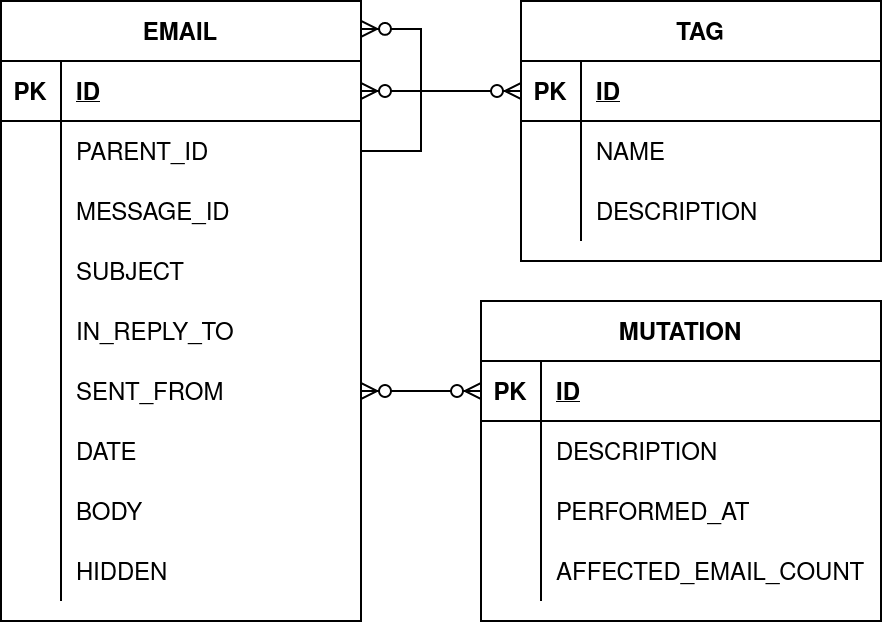
\includegraphics[width=0.5\textwidth]{img/simple_schema.png}
				\caption{A diagrammatic representation of the email dataset's relational schema.}
			\end{wrapfigure}
			The relational schema is the core of the email dataset, and defines how we operate on and organize the data. It is purposefully designed to be as simple as possible, to make it easy to use the dataset in a variety of applications and environments.
			
			The schema consists of three entities: \textit{emails}, \textit{tags}, and \textit{mutations} (although mutations are not strictly required).
			
			\textbf{Emails} are, as you'd probably expect, the entity that represents a single email message, sent by someone, in a mailing list. While emails \textit{do} have their own unique \texttt{MESSAGE\_ID} attribute\cite{rfc5322}, they are identified by an 8-byte integer primary key. This reduces the dataset size, improves search performance due to the monotonic nature of incrementing primary keys, and allows for easier referencing of emails by their id, instead of a long, randomly-generated message id.
			
			Also of note is an email's \texttt{PARENT\_ID}, which is a self-referencing foreign key that references another email entity by its id. This foreign key is the manifestation of the \textit{many-to-one} relationship between an email and its parent, where many "child" emails may refer to one parent email. The parent id is derived, when processing emails, from the email's "In-Reply-To" field. According to RFC 5322, the in-reply-to field, if present, must reference another email's message-id, and this format of replies forms the basis of an email thread's structure\cite{rfc5322}.
			
			\textbf{Tags} are entities which can be attached to any number of emails, to offer a method of categorizing emails. Originally in version 1 of the dataset format, tags were not entities but simple texts that were attached to each email, but it was discovered during the development of the tools for this research that there are several benefits to having tags as their own entities: the ability to edit a tag's name, provide a description, and reduce the total dataset size by referencing an 4-byte integer id instead of keeping a copy of a string for each tag applied to an email.
			
			There exists a \textit{many-to-many} relationship between \textbf{emails} and \textbf{tags}, which one could verbalize as, "A tag may be applied to many emails, and an email may have many tags applied to it."
			
			\textbf{Mutations} are entities that record some change to the dataset which is used as a historical record of how a the emails in a dataset are filtered or modified. Mutations are used at the discretion of any third-party application which interfaces with the EmailIndexer API, and are not required to be used.
			
			There exists a \textit{many-to-many} relationship between \textbf{mutations} and \textbf{emails}, which one could verbalize as, "A mutation may involve many emails, and an email may be involved in many mutations." It is not required that a mutation be linked to any emails.
			
		\subsubsection{Indexing with Lucene}
			Alongside the relational database resides the \texttt{index} directory, as mentioned at the start of this section. This contains the indexes produced by the \href{https://lucene.apache.org/}{Apache Lucene} indexing library when we build an index using the emails in the database. This index is then used for executing query searches over the database by users.
			
			For each email in the dataset, we index the following fields as non-stored string-type fields using the \texttt{DOCS\_AND\_FREQS\_AND\_POSITIONS} index options provided by Lucene\cite{apache-lucene}:
			\begin{itemize}
				\item The \texttt{SUBJECT} field.
				\item The \texttt{BODY} field.
			\end{itemize}
			In addition to these indexed fields, we store the email's id and pre-compute the \textit{root id} (id of the first email in the current email's thread), as these are essential for producing actionable results from any query search on the index.
			
	\subsection{Email Thread Structure}
		\begin{wrapfigure}{r}{0.4\textwidth}
			\label{fig:email-threads}
			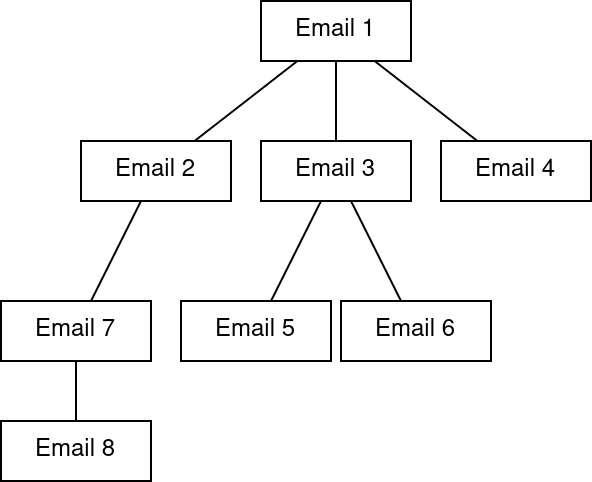
\includegraphics[width=0.4\textwidth]{img/email-threads.png}
		\end{wrapfigure}
	
		As previously mentioned, emails have a self-referencing \textit{many-to-one} relationship defined by their "In-Reply-To" field. It is important to understand the consequences of this structure, and how it impacts the dynamics of processing data. In any information system, a self-referencing, many-to-one relationship that an entity participates in, can be interpreted as a \textit{tree} data structure.
	
		Each email can be thought of as a node in the tree, where each reply to that email forms a branch. There is no limit to how wide or deep the tree can become, because there is no universal hard limit on the number of replies to an email, nor on how many replies may be sent in a thread.
		
		In previous research by den Boon, this natural tree structure of email threads was artificially flattened into a sequential list, presumably to facilitate more efficient methods of working with the data\cite{denboon}. However, in this research, the tree structure of the emails is preserved in the dataset, because it more accurately depicts how real users would navigate a set of emails using any number of existing programs, and therefore can provide a better model for determining the effectiveness of searches. This choice does come with some drawbacks, however.
		
		\begin{enumerate}
			\item Because emails form a tree structure, navigating the dataset is more computationally intensive, and more complex for a user, than if one could simply traverse a flat list.
			\item Analysis is more complex, due to the fact that most algorithms will need to incorporate tree traversal, either iteratively or recursively.
			\item Relational databases generally do not offer facilities for recursive fetching, which can lead to performance losses when processing large sets of emails.
		\end{enumerate}
	
		Despite the drawbacks, it is important to analyze and categorize emails in a format that does not lose the latent structural information contained in the email thread's tree itself. Furthermore, for this particular research, the volume of data and methods of analysis do not present any difficulties in terms of computational performance.
	
	\subsection{Email Dataset Browser}
		Now that we've prepared methods for fetching mailing lists, storing them, and indexing them for searching, the \href{https://github.com/ArchitecturalKnowledgeAnalysis/EmailDatasetBrowser}{Email Dataset Browser} tool is introduced as a means of first of all (obviously) browsing the set of all emails, searching over the emails using Lucene search queries, and categorizing emails using user-defined tags. This tool forms the basis for generating useful datasets with which we can perform analysis on the types of architectural knowledge that's found and annotated within the dataset.
		
		While this research builds off of the work of den Boon\cite{denboon}, it was determined to be infeasible to use the \textit{ArchDetector} tool developed for categorization.
		
		\begin{itemize}
			\item The Apache software foundation had updated their infrastructure for mailing list management, which broke compatibility with the tool.
			\item The tool treated email threads as a 1-dimensional sequential list, instead of a tree structure. The reasoning behind the decision to choose a tree structure is discussed in the previous section.
		\end{itemize}
	
		Instead, the Email Dataset Browser (or EDB for short) was developed as a simple interactive application that allowed users to navigate datasets, and apply tags to emails as an indication of how they're categorized.
		
		\begin{figure}[H]
			\label{fig:edb-screenshot}
			\centering
			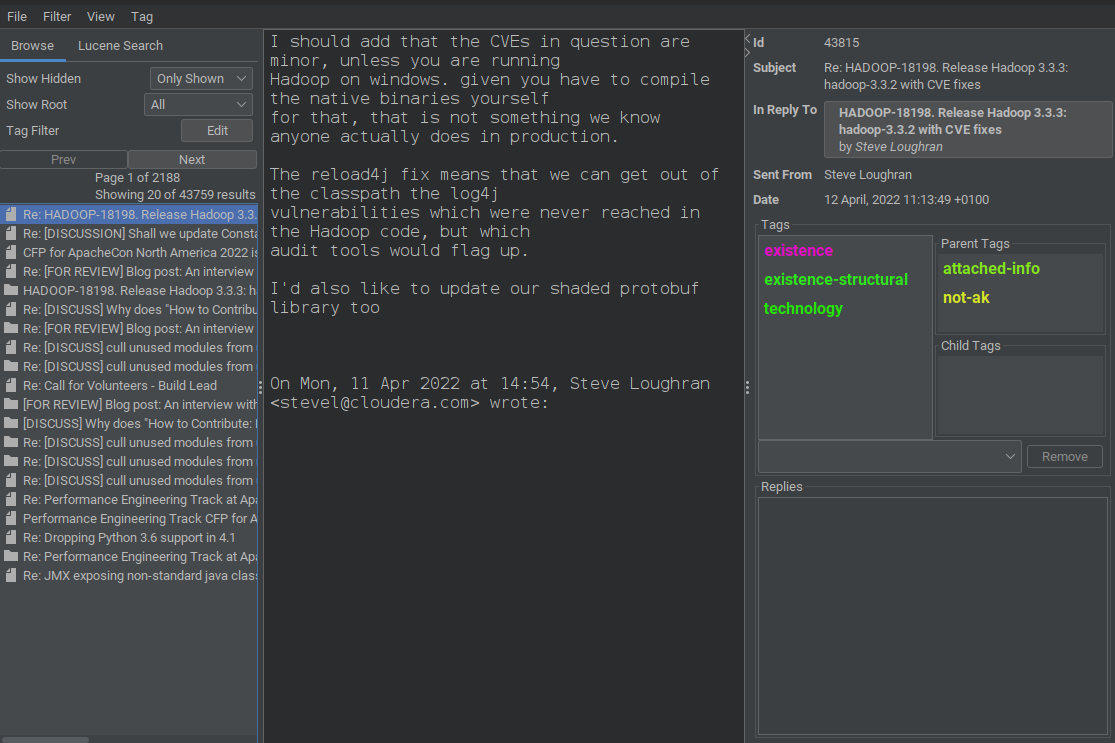
\includegraphics[width=\textwidth]{img/edb-screenshot.png}
			\caption{A screenshot of the email dataset browser app's main user interface, showing an email that has some tags.}
		\end{figure}
	
		We will not go into much detail on the implementation of this browser app; this is outside the scope of the research. Here are the main functionalities which it provides, that make the research possible:
		
		\begin{itemize}
			\item Navigate through all emails in a dataset.
			\item Apply Lucene search queries to a dataset and view the results.
			\item Add and remove tags that are applied to individual emails, to categorize them as containing architectural knowledge of a certain type.
			\item Export all or part of the dataset, in a variety of formats.
		\end{itemize}
	
		For more information on the implementation details of the EDB, please consult the \href{https://github.com/ArchitecturalKnowledgeAnalysis/EmailDatasetBrowser}{GitHub repository}.
	
	
	
	\subsection{Categorization Process}
		This study categorized the architectural knowledge contained in 1919 individual emails, spread across 188 different email threads from Hadoop, Cassandra, and Tajo developer mailing lists. This section provides an overview of how this was achieved.
		
		Email categorization happened in \textit{iterations}, where a selection of emails would be analyzed for the architectural knowledge they potentially contain, and a subset of this section was presented to the supervisor for verification. With each iteration, feedback and a broadening collection of examples helped to build the final \hyperref[sec:design-decisions]{list of design decisions} included in this paper, and already-categorized emails were revised under the new definitions. Additionally, repetitive patterns of easily-identifiable junk emails were discovered during these iterative reviews, and such emails were hidden from the dataset. The following criteria were grounds for the removal of emails from the working dataset:
		
		\begin{itemize}
			\item The subject or body of the email contained the phrase "call for papers".
			\item The email was sent by an automated process, like a Jenkins or mailing list bot program that sends automated test failure reports.
		\end{itemize}
	
		The rate at which email categorization can happen is a clear limiting factor to the scale of this study, because of the time requirements to develop an intuition for accurately identifying the design decisions in emails, and the time required to simply read such a volume of emails. This will be discussed further in the paper's conclusion.
		
	\subsection{Analysis}
		Once a reasonable sufficient number of emails were categorized, a set of analyses was developed to help illustrate the results, and how they pertain to the research questions.
		
		\subsubsection{Relevance}
			For multiple metrics in the analysis, we discuss an email or email thread's \textit{relevance}. This is a measure of how valuable such a result is, where those with high amounts of architectural knowledge should have a higher relevance than those who don't. And any email or thread containing no architectural knowledge should certainly have a relevance value of 0.
			
			For individual emails, we simply take an email's relevance value as 1 if it is categorized as containing at least one type of architectural design decision, or a value of 0 otherwise.
			
			Let $ e $ be an email, and $ |e| $ be the number of architectural tags applied to email $ e $. Then, we can compute the relevance $ rel(e) $ as follows:
			
			\begin{equation}
				\tag{Email Relevance}
				rel(e) =
				\begin{cases}
					1 & |e| > 0 \\
					0 & \text{otherwise}
				\end{cases}
				\label{eqn:relemail}
			\end{equation}
		
			For an entire email thread, the approach is more involved, as threads can contain wildly different amounts of architectural knowledge. We first compute the average number of tags among the top 10 threads containing the most architectural knowledge. This helps to give an unbiased indication of what we might consider to be the "best" threads. Let this average be referred to as $ rel_{max} $. More formally, let $ t_i $ be the $ i^{\text{th}} $ best thread, in terms of its number of architectural tags, and let $ |t_i| $ represent the number of tags of the $ i^{\text{th}} $ thread.
			
			\begin{equation}
				\tag{Email Thread Max Relevance}
				rel_{max} = \sum_{i=1}^{10} \frac{|t_i|}{10}
				\label{eqn:relmax}
			\end{equation}
			
			For a given thread $ t $ where $ |t| $ is the number of architectural tags contained in all emails in that thread, its relevance can be computed as follows:
			
			\begin{equation}
				\tag{Email Thread Relevance}
				rel(t) = min\Big(1, \frac{|t|}{rel_{max}}\Big)
				\label{eqn:relthread}
			\end{equation}
		
		\subsubsection{Lucene Search Precision}
			In order to answer the question of \textit{how effective} Lucene indexing and searching is to find relevant architectural knowledge, two metrics were used.
			
			First, a simple iterative precision metric is used to determine a search query's precision $ P_n $ for a search to find $ n $ emails or threads where $ rel_i $ is the relevance of the $ i^{\text{th}} $ email or thread:
			
			\begin{equation}
				\tag{Search Precision}
				P_n = \sum_{i = 1}^{n} \frac{p_i}{n}
				\text{ where } p_i =
				\begin{cases}
					1 & rel_i > 0 \\
					0 & rel_i <= 0
				\end{cases}
				\label{eqn:precision}
			\end{equation}
		
			This metric tells what ratio of results returned by a query contain some architectural knowledge, so it can be of use to describe how effective a search is at returning \textit{anything} of value, but does not account for the rank of elements in the search, nor the true relevance of email threads. This equation works for analyzing searches over individual emails, and searches over threads by obtaining $ rel_i $ using either \eqref{eqn:relemail} or \eqref{eqn:relthread}, respectively.
			
		\subsubsection{Normalized Discounted Cumulative Gain}
			A better metric that accounts for a result's \textit{rank} in addition to its relevance is the \href{}{Discounted Cumulative Gain}, and this helps us to model real-world user persistence in examining large result sets\cite{jarvelin}.

			\begin{equation}
				\tag{DCG}
				DCG_n = \sum_{i=1}^{n} \frac{rel_i}{log_2(i + 1)}
				\label{eqn:dcg}
			\end{equation}
			
			However, this metric may be wildly different depending on the query that's used. To compensate for this, we \textit{normalize} the cumulative gain by comparing the DCG to the best possible result that could be obtained, also known as the \textit{ideal} DCG\cite{stanfordslides}. Let $ REL_n $ be the list of the $ n $ most relevant documents in the dataset, ordered in descending order. Then we can compute the ideal DCG as follows:
			
			\begin{equation}
				\tag{IDCG}
				IDCG_n = \sum_{i=1}^{|REL_n|} \frac{rel_i}{log_2(i + 1)}
				\label{eqn:idcg}
			\end{equation}
		
			And once the IDCG is obtained, we can simply use this to normalize the DCG result produced by any query over the dataset.
			
			\begin{equation}
				\tag{NDCG}
				NDCG_n = \frac{DCG_n}{IDCG_n}
				\label{eqn:ndcg}
			\end{equation}
		
			In the end, we can use NDCG as a general metric to evaluate the effectiveness of a search query to produce \textit{highly relevant} results, with the \textit{most relevant results first}. In theory, we would like a perfect query for which the NDCG is computed as 1 for all $ n $\cite{denboon}.
			
		\subsubsection{N-Gram Patterns}
			Besides evaluating the effectiveness of the various query searches, we'd also like to answer questions about the content of architectural knowledge, and identifying patterns in how such knowledge appears can be key to understanding this. To that end, inspiration was taken from the \href{https://en.wikipedia.org/wiki/N-gram}{N-Gram} method for analyzing natural language. N-gram models have been used successfully in machine translation, speech recognition, entity detection, and information extraction\cite{google-ngram}. The n-gram approach can be applied to an email thread to find the most common ordered $ n $ length sequences of tags that appear in the dataset. Furthermore, Guthrie et al. demonstrated that \textit{skip-grams} (a technique where unmarked elements can be skipped) are effective at finding meaningful value from datasets without needing to increase the size of the dataset\cite{guthrie}.
			
			Therefore, we present a \hyperref[sec:pattern-algorithm]{recursive algorithm} for finding a list of all known sequences of email ids in a thread that correspond to one of many possible tag patterns, which can optionally be configured to skip non-architectural emails (generating a skip-gram model).
			
			First, the \texttt{patternSearchRecursive} method is defined to iterate over all tags on a given email, and for each tag, find any patterns that start with that tag. For any of those patterns, call the \texttt{findMatchingSequence} method and store the results in our \texttt{result} instance variable.
			
			The \texttt{findMatchingSequence} method will then recursively traverse an email thread from a starting email, until it finds a sequence that matches the given pattern of tags.
			
		\subsubsection{Co-Occurrence}
			N-grams are excellent at giving insight into the ordered patterns of architectural knowledge discussion, but a simpler co-occurrence metric can tell us what types of architectural knowledge most often appear together. For this, we just make a pass over all categorized emails, and increment a counter for each combination of tags that is encountered.
			
		\subsubsection{Aggregate Data}
			In addition to the above analyses, we will also provide a suite of simple aggregate analyses to be able to better visualize the data. This will include the following properties for each individual email:
			
			\begin{itemize}
				\item Body size: the total number of characters of the email's body.
				\item Word count: the total number of words in the email's body. Words are any sequence of text separated by one or more whitespace characters.
			\end{itemize}
		
			And for email threads, the following additional properties will be examined:
			
			\begin{itemize}
				\item Thread size: the total number of emails in a thread.
				\item Participant count: the total number of all unique participants in a thread.
			\end{itemize}

\section{Results}
	In this study, 1919 individual emails, in 188 unique email threads, were categorized according to the architectural design decisions they contained. Furthermore, this set contains the top 75 email threads from each of the four provided \hyperref[sec:queries]{Lucene search queries}. We will now illustrate the results of this effort, and attempt to substantiate answers to the posed \hyperref[sec:research-questions]{research questions}.
	
	\footnotesize
	Note that all data, plots, and other graphics that were programmatically generated, have their \href{https://github.com/ArchitecturalKnowledgeAnalysis/EmailDatasetReportGen}{source code available on GitHub.com}.
	\normalsize
	
	\subsection{Kinds of Architectural Design Decisions}
		To answer the first and second research questions, we can look at the total number of emails (and threads) that have been categorized under each type of \hyperref[sec:design-decisions]{architectural design decision}.
		
		\begin{figure}[H]
			\centering
			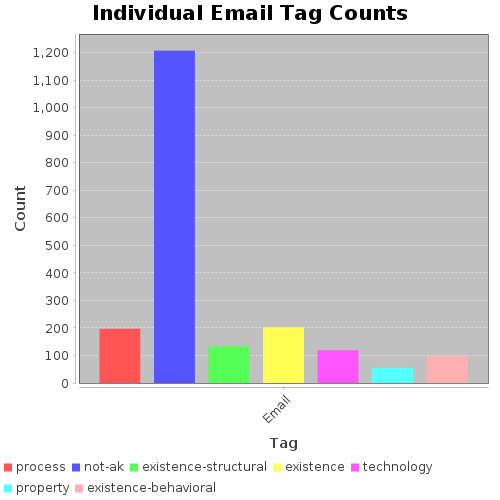
\includegraphics[width=0.7\textwidth]{report/overview/individual_email_tag_count.png}
			\caption{The total number of emails with each type of tag.}
			\label{fig:emailtagcount}
		\end{figure}
	
		From figure \ref{fig:emailtagcount} we can clearly see that the majority of emails contain no architectural knowledge at all, and by a large margin. However, we also see some interesting variation in what kinds of architectural design decisions do exist, with existence being the most common, followed closely by process decisions.
	
		Looking at the results for threads in figure \ref{fig:threadtagcount}, the outlook isn't quite so depressing. Despite the fact that yet again, \textit{most} threads generally don't have architectural knowledge, a large portion of threads \textit{do} contain a significant number of identified design decisions. Again, existence decisions are the most popular, but thereafter it is evident that there is a relatively large number of threads discussing technology decisions, while fewer process discussions than one would expect if extrapolating the individual email data.
	
		\begin{figure}[H]
			\centering
			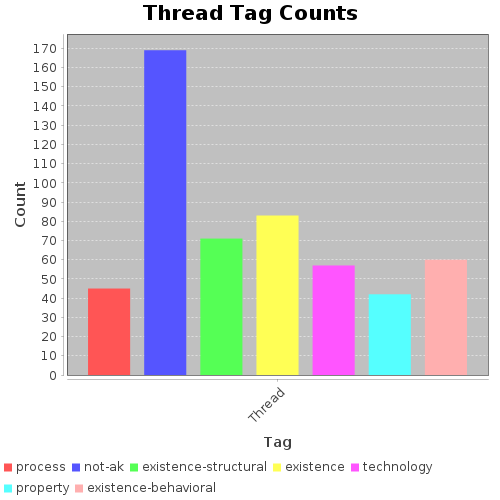
\includegraphics[width=0.7\textwidth]{report/overview/thread_tag_count.png}
			\caption{The total number of threads that contain each at least one email with a given tag.}
			\label{fig:threadtagcount}
		\end{figure}
	
		The reduced frequency of process discussions at the thread level, juxtaposed with the increased frequency at the individual email level, indicates that there exists a fewer number of threads discussing development processes, \textit{but} those threads which \textit{do} discuss processes, generally contain more emails. We can see this difference illustrated further in figure \ref{fig:threadsize}, which plots the distribution of thread sizes for threads containing various tags.
		
		Conversely, there are proportionately more threads discussing technology than there are individual emails, and again this can be explained by the nature of such discussions. Conversations about technologies tend to be shorter than other conversations about the actual architecture of a system, probably because there is a lesser need to reason about and qualify decisions compared to the system's own components.
		
		\begin{figure}[H]
			\centering
			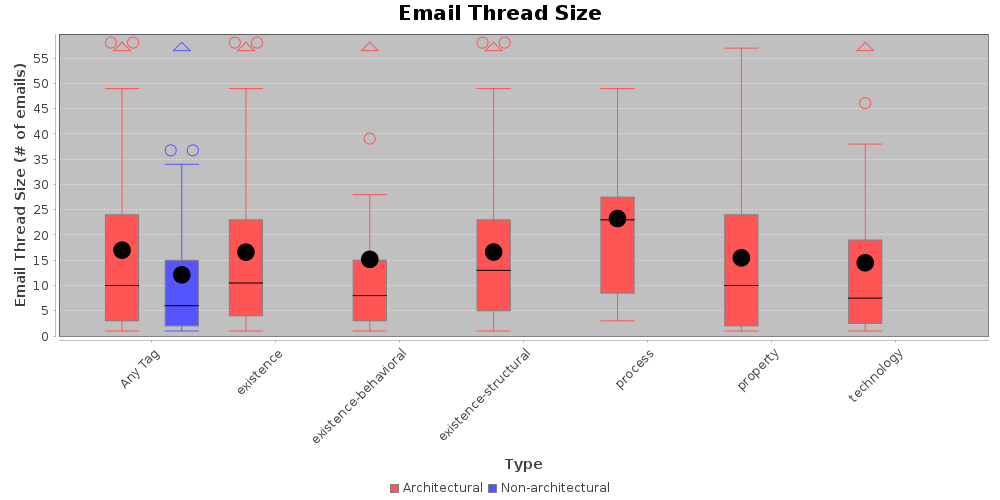
\includegraphics[width=0.8\textwidth]{report/characteristics/thread_size.png}
			\caption{Boxplot showing the distribution of thread size for different tags.}
			\label{fig:threadsize}
		\end{figure}
	
		\begin{figure}[H]
			\centering
			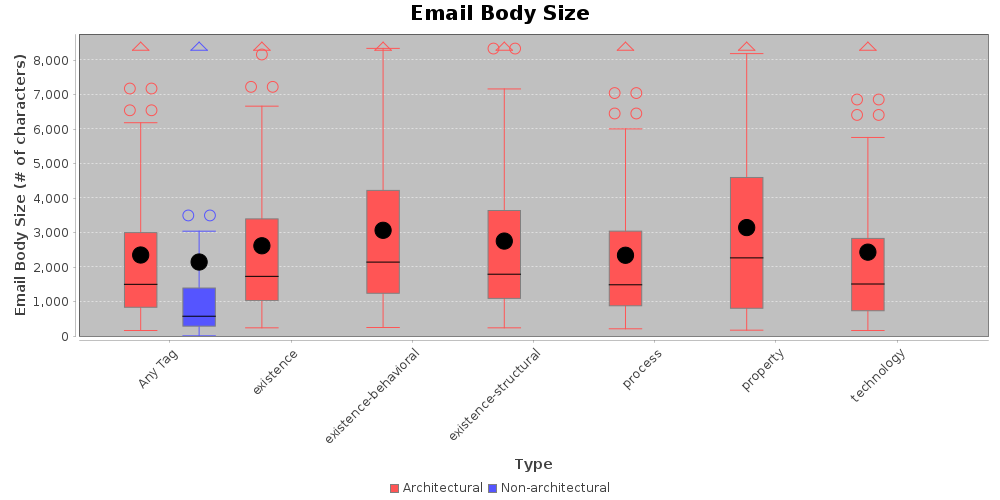
\includegraphics[width=0.8\textwidth]{report/characteristics/body_size.png}
			\caption{Boxplot showing the distribution of body sizes of emails for different tags.}
			\label{fig:bodysize}
		\end{figure}
	
		\begin{figure}[H]
			\centering
			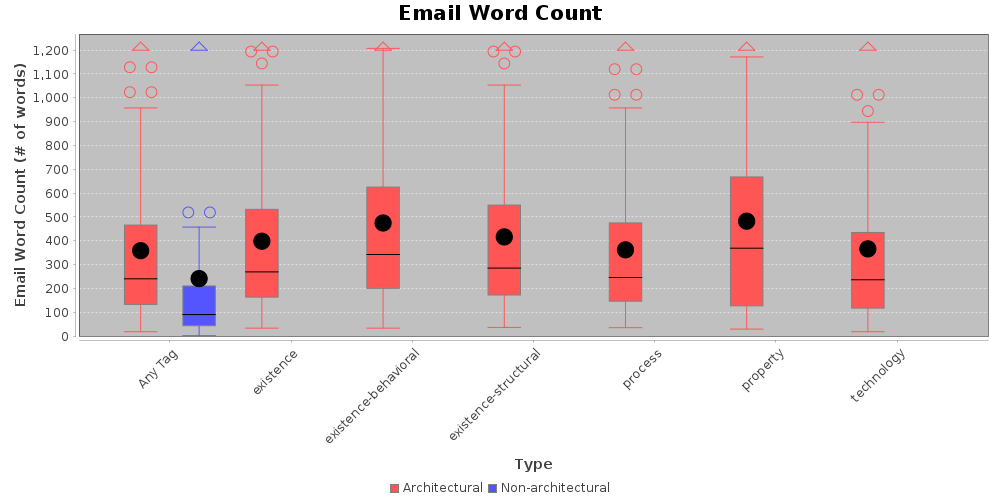
\includegraphics[width=0.8\textwidth]{report/characteristics/word_count.png}
			\caption{Boxplot showing the distribution of word counts of emails for different tags.}
			\label{fig:wordcount}
		\end{figure}
		
		The \eqref{eqn:relthread} equation provides some insight into how often architectural knowledge appears. We observe a roughly linear gradient from a relevance of 0.1 to a relevance of 1.0, and again we see that a plurality of email threads are mostly irrelevant in terms of their architectural knowledge content.
		
		\begin{figure}[H]
			\centering
			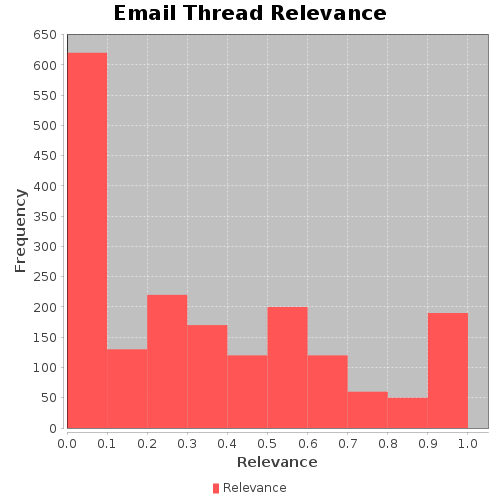
\includegraphics[width=0.7\textwidth]{report/overview/relevances.png}
			\caption{Histogram that shows the distribution of the relevance of all email threads.}
			\label{fig:threadrelevance}
		\end{figure}
	
	\subsection{Patterns of Design Decisions}
		To determine if and what sort of patterns exist in progression of architectural design decisions through an email thread, a series of n-gram and co-occurrence analyses were performed. We will first discuss what patterns exist, and then consult a few cases to try and understand why those patterns exist.
		
		\begin{table}[H]
			\centering
			\caption{The top 5 most common 2-gram sequences.}
			\begin{tabular}{|l|l|}
				\hline
				\textbf{Pattern} & \textbf{Count} \\ \hline
				property $ \rightarrow $ existence & 18 \\ \hline
				technology $ \rightarrow $ existence & 17 \\ \hline
				existence $ \rightarrow $ process & 17 \\ \hline
				existence $ \rightarrow $ technology & 16 \\ \hline
				existence $ \rightarrow $ property & 15 \\ \hline
			\end{tabular}
		\end{table}
		
		\begin{table}[H]
			\centering
			\caption{The top 5 most common 2-gram sequences, skipping non-architectural emails between tags.}
			\begin{tabular}{|l|l|}
				\hline
				\textbf{Pattern} & \textbf{Count} \\ \hline
				property $ \rightarrow $ existence & 30 \\ \hline
				existence $ \rightarrow $ property & 30 \\ \hline
				existence $ \rightarrow $ process & 29 \\ \hline
				technology $ \rightarrow $ existence & 28 \\ \hline
				existence $ \rightarrow $ technology & 27 \\ \hline
			\end{tabular}
		\end{table}
	
		Already with just the 2-gram model, it is clear that there is a sort of bidirectional relationship between property and existence decisions, and between existence and technology decisions. Furthermore, the model indicates that there is not a strong directionality in the patterns, since most pairs have a similar frequency with both orientations. The skip-gram technique does lead to more abundant results, but there may be a slightly reduced accuracy\cite{guthrie}, in that an arbitrary number of intermediate emails have been skipped, thus the application of a skip-gram model may not be as reliable as the non-skip, but seems to perform better without needing a larger dataset.
	
		\begin{table}[H]
			\centering
			\caption{The top 5 most common 3-gram sequences.}
			\begin{tabular}{|l|l|}
				\hline
				\textbf{Pattern} & \textbf{Count} \\ \hline
				property $ \rightarrow $ existence $ \rightarrow $ process & 4 \\ \hline
				existence $ \rightarrow $ property $ \rightarrow $ technology & 3 \\ \hline
				technology $ \rightarrow $ existence $ \rightarrow $ process & 2 \\ \hline
				property $ \rightarrow $ technology $ \rightarrow $ existence & 2 \\ \hline
				property $ \rightarrow $ technology $ \rightarrow $ process & 2 \\ \hline
			\end{tabular}
		\end{table}
		
		\begin{table}[H]
			\centering
			\caption{The top 5 most common 3-gram sequences, skipping non-architectural emails between tags.}
			\begin{tabular}{|l|l|}
				\hline
				\textbf{Pattern} & \textbf{Count} \\ \hline
				property $ \rightarrow $ existence $ \rightarrow $ process & 6 \\ \hline
				technology $ \rightarrow $ existence $ \rightarrow $ process & 6 \\ \hline
				existence $ \rightarrow $ process $ \rightarrow $ property & 5 \\ \hline
				existence $ \rightarrow $ property $ \rightarrow $ technology & 4 \\ \hline
				property $ \rightarrow $ technology $ \rightarrow $ existence & 4 \\ \hline
			\end{tabular}
		\end{table}
	
		Given that the dataset consists of nearly 2,000 categorized emails, the results of the 3-gram models show that there is no abundant evidence for any highly structured patterns of discussion. The skip-gram model does not offer much improvement, and because of this, we will discard the 3-gram models from further discussion as being irrelevant.
	
		\begin{table}[H]
			\centering
			\caption{Co-occurrence frequency for pairs of tags.}
			\begin{tabular}{|l|l|}
				\hline
				\textbf{Pattern} & \textbf{Count} \\ \hline
				existence, property & 31 \\ \hline
				existence, technology & 25 \\ \hline
				existence, process & 14 \\ \hline
				process, technology & 9 \\ \hline
				property, technology & 8 \\ \hline
				process, property & 8 \\ \hline
			\end{tabular}
			\label{fig:2co-occurrence}
		\end{table}
	
		The co-occurrence data shown in figure \ref{fig:2co-occurrence} reinforces the previous claim about a relationship between the existence and property decisions, and existence and technology decisions. Now that it is clear that such relationships do exist, we will discuss the possible motivation for the existence of these relationships.
		
		Regarding the existence $ \leftrightarrow $ property relationship, several cases indicate that this happens when a participant begins a high-level proposal or discussion on adding a new component, or integrating a subsystem into the main architecture. This tends to initiate a conversation with one or more property decisions, as users and developers debate on the existing and new properties of the system, and once this is resolved, concrete components or connections between components are proposed.
		
		For example,
		
		\begin{itemize}
			\item The email thread with subject \texttt{[DISCUSS] CEP 19: Trie memtable implementation} begins with a proposal to contribute a new implementation of a memtable to the Cassandra project. The initial email provides some overarching objectives that the new implementation wishes to achieve in terms of performance. A follow-up email expands upon this proposal with some details about the implementation, which includes a modification to an API and an update to Cassandra's configuration scheme.
			\item A Hadoop \texttt{Security Design Lounge Session} thread begins by addressing some concerns regarding Hadoop's authentication and security, and identifies some basic requirements for the system's integration support and security audit needs. Various Hadoop contributors and users respond with their opinions on the matter, and some make very explicit recommendations for how to structure the project such that authentication can be made pluggable.
		\end{itemize}
	
		In the other common bidirectional case with existence $ \leftrightarrow $, we see a similar pattern of a proposal followed by a rich discussion. For this relationship, however, proposals often directly or indirectly mention third-party technologies, and ensuing conversation includes a series of emails that evaluate the value of integrating such technologies into the architecture.
		
		For example,
		
		\begin{itemize}
			\item A thread discussing the replacement of Cassandra's command-line interface framework in the various auxiliary tools Cassandra ships with. The initial email is phrased as a sort of "call for ideas" for suitable replacements. Replies discuss the benefits and drawbacks of various popular CLI libraries and how they'll affect the existing architecture.
			\item In the \texttt{[DISCUSS] Secure Hadoop without Kerberos} thread, a developer begins by explaining the drawbacks of using the Kerberos authentication system for Hadoop, and several developers respond with information about comparable alternative authentication schemes like OpenID Connect or ActiveDirectory, and further discuss how these could be integrated into Hadoop with the addition of certain new components.
		\end{itemize}
	
	\subsection{Search Effectiveness}
		To determine the effectiveness of our four \hyperref[sec:queries]{queries} at finding relevant emails and threads rich in architectural design decisions, we will use both the \hyperref[eqn:precision]{precision} and \hyperref[eqn:ndcg]{NDCG} as metrics to evaluate over each query.
		
		From figure \ref{fig:precisionall} we can see immediately that all queries generally perform quite well in terms of their precision. Recall that the precision is a measure of the average ratio of returned results that contain architectural knowledge, meaning that all four queries perform slightly above 50\%. Initially, the \textit{decision factors} query performs better, followed by the \textit{rationale} query from $ n = 7 $ onward. The \textit{reusable solutions} and \textit{components and connectors} queries in contrast perform relatively poorly in the initial results, but precision improves as $ n $ approaches 20. However, it should be noted that the initial performance is highly unstable and slight variations in the content of emails may completely alter the first few results, and so practically we should only consider evaluating a query based on its total precision over a greater $ n $.
		
		In figure \ref{fig:ndcgall}, the NDCG metric is visualized for the four queries. The graph is less chaotic than the precision graph, and we can see a more organized trend line for three of queries, while the \textit{reusable solutions} performs consistently at the lowest level. Again, \textit{decision factors} and \textit{rationale} perform well initially, and in this metric, they continue to provide the best performance, albeit by a tiny margin. Despite the fact that the NDCG metric "discounts" results at lower ranks in the result, the queries appear to improve in performance slightly as the result set grows larger. This could indicate that the factor by which we discount lower-ranked results is too weak, or that the queries are simply not effective at ranking highly-relevant results appropriately.
		
		\begin{figure}
			\centering
			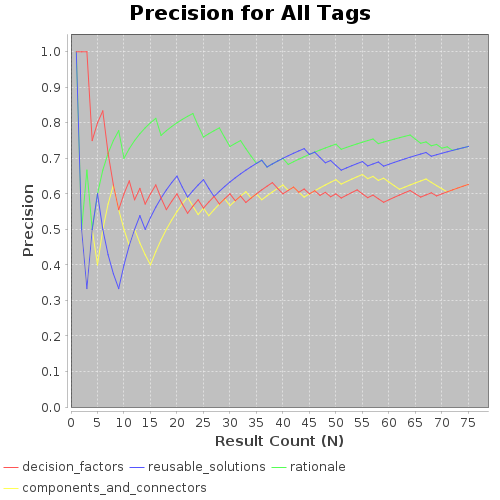
\includegraphics[width=\textwidth]{report/precision/precision_all.png}
			\caption{Precision metric with thread relevance computed using all architectural design decision tags, for all queries.}
			\label{fig:precisionall}
		\end{figure}
		
		\begin{figure}
			\centering
			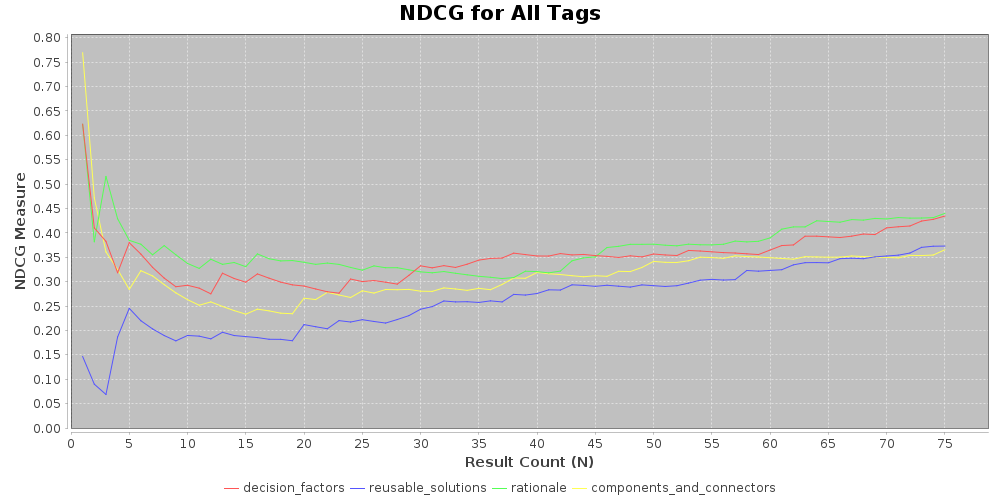
\includegraphics[width=\textwidth]{report/precision/ndcg_all.png}
			\caption{NDCG metric with thread relevance computed using all architectural design decision tags, for all queries.}
			\label{fig:ndcgall}
		\end{figure}
	
		While the focus in this study is on evaluating the effectiveness of queries in a real-world context that's similar to how a user would really search for knowledge, we also include precision and NDCG measures when using the queries to search over individual emails, to compare with the thread-based search. This type of search benefits from a larger dataset volume, as we have roughly 10 times as many fully categorized emails as threads, but does not accurately depict a typical human search, since it removes context from the search results by returning fragmented bits of information from many different conversations. Generally the searches perform worse over individual emails than they do over threads, with both precision and NDCG values remaining below $ 0.4 $ for almost the entirety of the query results, and degrading as $ n $ increases. However, it appears that the \textit{reusable solutions} query, which performed most poorly in the thread-based precision and NDCG metrics, tends to perform at or near the best of all the queries for individual emails.
		
		\begin{figure}
			\centering
			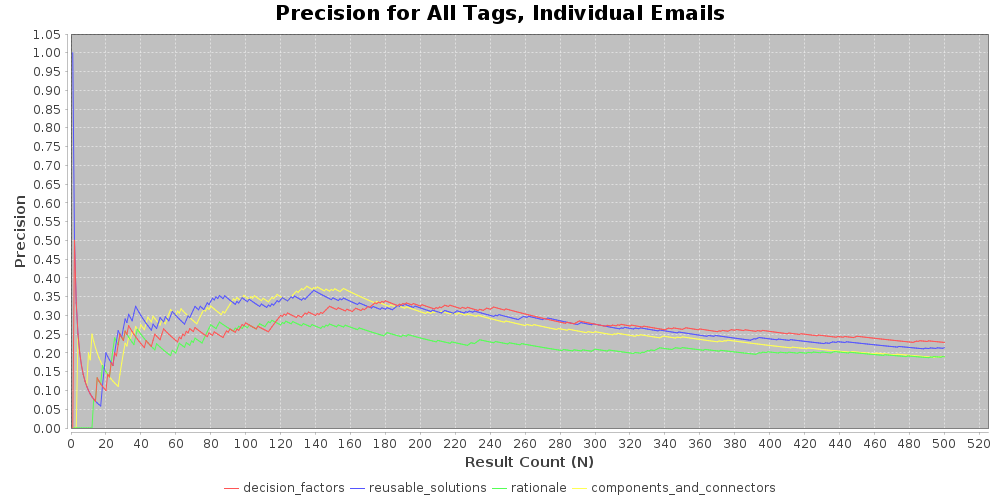
\includegraphics[width=\textwidth]{report/precision/precision_all_emails.png}
			\caption{Precision metric with email relevance computed using all architectural design decision tags, for all queries.}
			\label{fig:precisionemailall}
		\end{figure}
		
		\begin{figure}
			\centering
			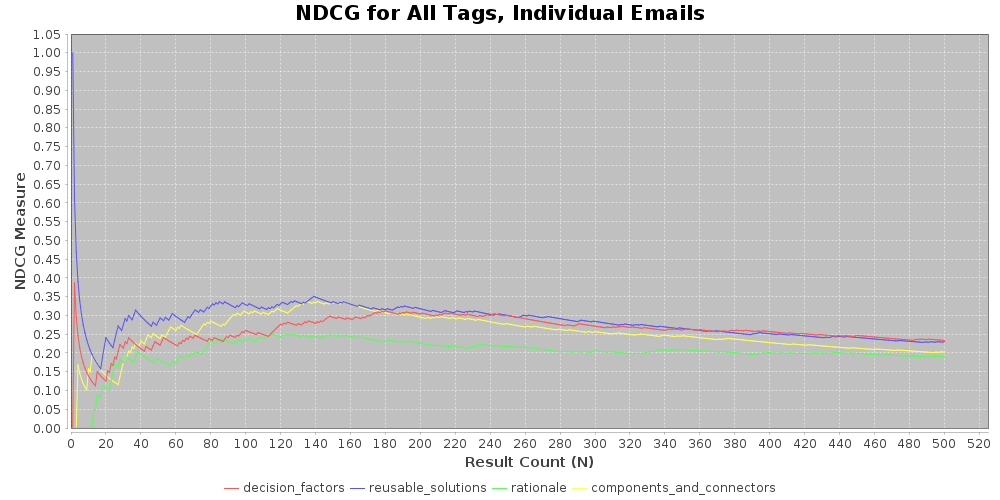
\includegraphics[width=\textwidth]{report/precision/ndcg_all_emails.png}
			\caption{NDCG metric with email relevance computed using all architectural design decision tags, for all queries.}
			\label{fig:ndcgemailall}
		\end{figure}

\section{Conclusion}
	In this study, we prepared tools to fetch and process mailing lists, and prepared a categorized dataset containing 1919 emails in 188 unique email threads, to determine what types of architectural knowledge exists in open-source software development mailing lists. The results of a varied set of analyses over this dataset tell us first and foremost that \textit{most} emails in such mailing lists do not contain useful architectural design decisions, but that a large proportion of email threads \textit{do} contain architectural design decisions. There exists a strong relationship between existence decisions and both technology and property decisions, as a natural consequence of the flow of a conversation from proposal to an evaluation of alternative solutions, to choosing an accepted solution.
	
	From applying Apache Lucene search queries to the dataset, the precision and NDCG metrics for both thread-based and individual email results indicate that the current search implementation is not effective for finding a sufficient amount of architectural knowledge, when compared to similar metrics performed by den Boon\cite{denboon} where queries achieved NDCG measures of greater than $ 0.9 $ over 100 results.
	
	Open-source software development mailing lists, as shown by this research, present ample opportunity for extracting architectural knowledge, and we have shown that contextual patterns in the types of design decisions can be used to further aid in searching. However, the search methods used in this study, or the metrics used to grade them, were insufficient to conclude that keyword-based Lucene queries are an effective tool for extracting that knowledge. More work is needed to improve how the queries operate over email threads, how to compute a more accurate relevance measure, and improved metrics are needed to be able to better differentiate the performance of different queries.
	
	\subsection{Threats to Validity}
		Despite the researcher's best efforts, the data in this paper could be subject to a number of faults, and it is important that the reader acknowledge these before pressing onward with any research that depends on these results.
		
		The researcher is a single student whose practical experience does not overlap much with the realm of architectural knowledge identification and extraction. The researcher did iteratively develop a sense of intuition for the design decisions through many weeks of supervised email categorization, but this is still prone to the occasional error. Fatigue may play a role in producing lower-quality results, as multiple hours of reading emails tends to drain the mind of all its vitality.
		
		The indexing and searching implementation may not be optimal for email threads, as no general solution exists for this, given that mailing lists are usually navigated chronologically by their users. The \ref{eqn:relthread} equation may not be optimal for computing a truly useful relevance value for an email thread.
		
	\subsection{Future Work}
		This study provides a solid basis for identifying the types and amount of architectural knowledge that can be found in open-source software development mailing lists, but is far from an exhaustive resource on the matter. Additional research is needed to further expand on the data with additional mailing lists from other open-source communities that focus on different types of software. While we explored the patterns in how architectural design decisions are made, our research was limited to exclusively the content of the emails themselves, and there are many examples where the discussion in an email is migrated to a Jira or GitHub issue tracker, and the reasons for these "jumps" between media has not yet been explored, nor the patterns which might exist between discussions on either end.
		
		While more work can be done to improve the indexing and searching implementation, and the queries used by it, research by Bhat et al.\cite{bhat} shows that there is promise in designing machine learning models to automatically extract architectural knowledge. The data in this study can be incorporated into training data for such models.
		
		The tools developed for this study are rudimentary in nature, but have been developed to the best of the researcher's abilities to be future-proof and open to expansion and re-use, and we encourage others to build on their capabilities. Currently, the \href{https://github.com/ArchitecturalKnowledgeAnalysis/EmailDownloader}{EmailDownloader} utility supports only Apache Software Foundation mailing lists, but could be expanded easily to support others as well. The \href{https://github.com/ArchitecturalKnowledgeAnalysis/EmailIndexer}{EmailIndexer} utility currently only supports the H2 database implementation, which offers limited concurrency when operating in embedded mode, and this can be improved to allow for multi-user systems where many people can contribute to a single dataset's information at once. And finally, the \href{https://github.com/ArchitecturalKnowledgeAnalysis/EmailDatasetBrowser}{EmailDatasetBrowser} application could be expanded to include real-time analytics and improved search interfaces.

\section{References}
	\printbibliography[heading=none]
	\newpage

\section{Appendix}
	This section will contain larger bits of text or code or figures that aren't well suited to being placed inside the body of the paper. They may be referenced throughout the body of the paper. Note that not all source code for the various tools and analyses are included here, due to the impracticality of distributing such a large amount of source code. For the complete suite of software used in this study, please visit the \href{https://github.com/ArchitecturalKnowledgeAnalysis}{ArchitecturalKnowledgeAnalysis} organization on GitHub.
	
	\newpage
	\subsection{Lucene Keyword Queries}
		\label{sec:queries}
		This section contains four keyword-based Lucene search queries provided by Mohamed Soliman, as derived from previous research for use in this project. You may consult \href{https://lucene.apache.org/core/9_2_0/queryparser/org/apache/lucene/queryparser/classic/package-summary.html#package.description}{Apache Lucene's documentation} for a reference of the syntax used in these queries.
		
		\begin{table}[H]
			\begin{tabular}{p{0.4\linewidth} p{0.55\linewidth}}
				Decision Factors &
				\tiny
				\texttt{actor* availab* budget* business case* client* concern* conform* consisten* constraint* context* cost* coupl* customer* domain* driver* effort* enterprise* environment* experience* factor* force* function* goal* integrity interop* issue* latenc* maintain* manage* market* modifiab* objective* organization* performance* portab* problem* purpose* qualit* reliab* requirement* reus* safe* scal* scenario* secur* stakeholder* testab* throughput* usab* user* variability limit* time cohesion efficien* bandwidth speed* need* compat* complex* condition* criteria* resource* accura* complet* suitab* complianc* operabl* employabl* modular* analyz* readab* chang* encapsulat* transport* transfer* migrat* mova* replac* adapt* resilienc* irresponsib* stab* toleran* responsib* matur* accountab* vulnerab* trustworth* verif* protect* certificat* law* flexib* configur* convent* accessib* useful* learn* understand*}
				\\
				Reusable Solutions &
				\tiny
				\texttt{action* adapt* alloc* alternativ* approach* asynch* audit* authentic* authoriz* balanc* ballot* beat bridg* broker* cach* capabilit* certificat* chain* challeng* characteristic* checkpoint* choice* cloud composite concrete concurren* confident* connect* credential* decorat* deliver* detect* dual* echo encapsulat* encrypt* esb event* expos* facade factor* FIFO filter* flyweight* framework* function* handl* heartbeat* intermedia* layer* layoff* lazy load lock* mandator* measure* mechanism* memento middleware minut* monitor* mvc observ* offer* opinion* option* orchestrat* outbound* parallel passwords pattern* peer* period* piggybacking ping pipe* platform* point* pool principle* priorit* processor* profil* protect* protocol* prototyp* provid* proxy publish* recover* redundan* refactor* removal replicat* resist* restart restraint* revok* rollback* routine* runtime sanity* schedul* sensor* separat* session* shadow* singleton soa solution* spare* sparrow* specification* stamp* standard* state stor* strap strateg* subscrib* suppl* support* synch* tactic* task* technique* technolog* tier* timer* timestamp* tool* trail transaction* uml unoccupied* view* visit* vot* wizard* worker*}
				\\
				Components and Connectors &
				\tiny
				\texttt{access* allocat* application* architecture* artifact* attribute* behav* broker* call* cluster* communicat* component* compos* concept* connect* consist* construct* consum* contain* control* coordinat* core criteria* data database* decompos* depend* design* diagram* dynamic element* engine* entit* event* exchang* exist* external filter* function* hardware* independ* information infrastructure input* instance* integr* interac* internal item* job* layer* link* load* logic* machin* memor* messag* model* modul* node* operat* outcom* output* part* peer* platform* port* process* produc* program* project* propert* provid* publish* read* relat* request* resourc* respon* scope separate server* service* shar* source* stor* structur* subscrib* support* system* target* transaction* trigger* runtime realtime network* thread* parallel notif* distribut* backend* frontend* central* persist* queue* concurren* middleware* provid* suppl*}
				\\
				Rationale &
				\tiny
				\texttt{advantag* alternativ* appropriate assum* benefit* better best caus* choic* choos* complex* condition* critical decid* decision* eas* evaluat* hard* quick* rational* reason* risk* simpl* strong* tradeoff weak* rational* disadvantag* comparison* pros cons good differen* slow* lightweight overkill* recommend* suggest* propos* outperform* important* versus vs contrast* distinct* fast* heav* boost* drawback* option*}
				\\
			\end{tabular}
		\end{table}
	
	\newpage
	\subsection{Email Dataset Schema}
		\label{sec:dataset-schema}
		The following SQL snippet defines the relational schema which is used for email datasets in version 2 of EmailIndexer API.
		
		\footnotesize{This DDL script is written using the H2 dialect of SQL.}
		
		\begin{minted}{sql}
CREATE TABLE EMAIL (
	ID BIGINT PRIMARY KEY AUTO_INCREMENT,
	PARENT_ID BIGINT NULL DEFAULT NULL REFERENCES EMAIL(ID)
		ON UPDATE CASCADE ON DELETE SET NULL,
	MESSAGE_ID VARCHAR(255) UNIQUE,
	SUBJECT VARCHAR(1024),
	IN_REPLY_TO VARCHAR(255),
	SENT_FROM VARCHAR(255),
	DATE TIMESTAMP WITH TIME ZONE,
	BODY LONGTEXT,
	HIDDEN BOOL NOT NULL DEFAULT FALSE,
	CHECK (PARENT_ID IS NULL OR PARENT_ID <> ID)
);
CREATE INDEX IDX_EMAIL_DATE ON EMAIL(DATE);
CREATE INDEX IDX_EMAIL_HIDDEN ON EMAIL(HIDDEN);

CREATE TABLE TAG (
	ID INTEGER PRIMARY KEY AUTO_INCREMENT,
	NAME VARCHAR(255) UNIQUE,
	DESCRIPTION MEDIUMTEXT NULL DEFAULT NULL
);
CREATE INDEX IDX_TAG_NAME ON TAG(NAME);

CREATE TABLE EMAIL_TAG (
	EMAIL_ID BIGINT NOT NULL REFERENCES EMAIL(ID)
		ON UPDATE CASCADE ON DELETE CASCADE,
	TAG_ID INTEGER NOT NULL REFERENCES TAG(ID)
		ON UPDATE CASCADE ON DELETE CASCADE,
	PRIMARY KEY (EMAIL_ID, TAG_ID)
);

CREATE TABLE MUTATION (
	ID BIGINT PRIMARY KEY AUTO_INCREMENT,
	DESCRIPTION LONGTEXT NOT NULL,
	PERFORMED_AT TIMESTAMP WITH TIME ZONE NOT NULL DEFAULT CURRENT_TIMESTAMP(0),
	AFFECTED_EMAIL_COUNT BIGINT NOT NULL DEFAULT 0
);
CREATE INDEX IDX_MUTATION_DATE ON MUTATION(PERFORMED_AT);

CREATE TABLE MUTATION_EMAIL (
	MUTATION_ID BIGINT NOT NULL REFERENCES MUTATION (ID)
		ON UPDATE CASCADE ON DELETE CASCADE,
	EMAIL_ID BIGINT NOT NULL REFERENCES EMAIL(ID)
		ON UPDATE CASCADE ON DELETE CASCADE,
	PRIMARY KEY (MUTATION_ID, EMAIL_ID)
);
		\end{minted}
	
	\newpage
	\subsection{N-Gram Pattern Finder Algorithm}
		\label{sec:pattern-algorithm}
		
		\begin{minted}{java}
private void patternSearchRecursive(long emailId) {
	List<String> tags = tagRepo.getTags(emailId).stream().map(Tag::name).toList();
	for (String tag : tags) {
		for (List<String> pattern : result.patterns()) {
			if (pattern.size() > 0 && pattern.get(0).equals(tag)) {
				List<List<Long>> matchingSequences = findMatchingSequences(emailId, pattern);
				result.resultMap().get(pattern).emailIdSequences().addAll(matchingSequences);
			}
		}
	}
	for (long replyId : emailRepo.findAllReplyIds(emailId)) {
		patternSearchRecursive(replyId);
	}
}
		\end{minted}
		
		\begin{minted}{java}
private List<List<Long>> findMatchingSequences(long emailId, List<String> pattern) {
	if (pattern.size() <= 0) return new ArrayList<>();
	List<String> tags = tagRepo.getTags(emailId).stream().map(Tag::name).toList();
	boolean thisEmailMatches = tags.contains(pattern.get(0));
	List<List<Long>> sequences = new ArrayList<>();
	if (thisEmailMatches) {
		if (pattern.size() == 1) {
			List<Long> sequence = new ArrayList<>();
			sequence.add(emailId);
			sequences.add(sequence);
		} else {
			for (long replyId : emailRepo.findAllReplyIds(emailId)) {
				List<List<Long>> replySequences = findMatchingSequences(replyId, pattern.subList(1, pattern.size()));
				for (List<Long> sequence : replySequences) {
					sequence.add(0, emailId);
					sequences.add(sequence);
				}
			}
		}
	} else if (skipNotAk && tags.stream().anyMatch(ReportGen.NEGATIVE_TAGS::contains)) {
		for (long replyId : emailRepo.findAllReplyIds(emailId)) {
			List<List<Long>> replySequences = findMatchingSequences(replyId, pattern);
			sequences.addAll(replySequences);
		}
	}
	return sequences;
}
		\end{minted}
		
		\footnotesize
		Note that this is an excerpt from source code available online at the \href{https://github.com/ArchitecturalKnowledgeAnalysis/EmailDatasetReportGen/blob/fed23ead1039c99524e5dba7e797e942a55254ba/src/main/java/nl/andrewl/emaildatasetreportgen/pattern/NGramPatternSearcher.java}{EmailDatasetReportGen} repository.
		\normalsize

\end{document}